\documentclass[tikz,convert=false]{standalone}

\usepackage{tikz}
\usepackage{ifthen}
\usetikzlibrary{arrows}


\begin{document}

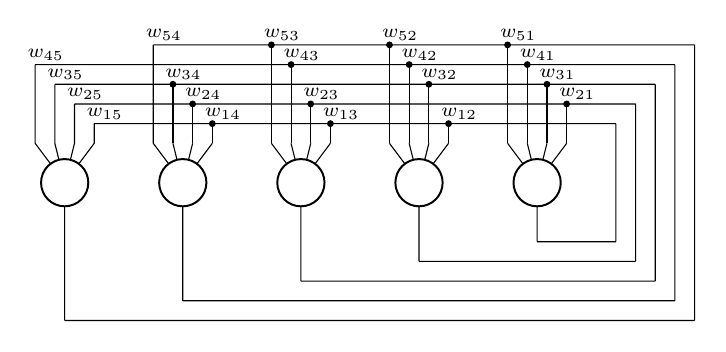
\begin{tikzpicture}
[connection/.style={-,shorten >=0.5pt},
invisible/.style={draw=none,fill=none,inner sep=0pt,minimum size=0mm,line width=0mm},
neuron/.style={circle,draw=black,fill=white,inner sep=0pt,minimum size=6mm,line width=0.25mm},
connectionUnion/.style={circle,draw=black,fill=black,inner sep=0pt,minimum size=0.6mm,line width=0.25mm},]

\def \numNeurons {5}
\def \spaceBetweenNeurons {1.5}
\def \spaceBetweenConnections {0.25}
\def \verticalDistanceToConnections {0.5}
\def \verticalOffset {0.75}
\def \weightVerticalPosOffset {0.125}
\def \weightHorizontalPosOffset {0.135}
\def \horizontalOffset {0.25}

\pgfmathparse{int(\numNeurons-1)}
\let\numConnectionsPerNeuron\pgfmathresult    

% LAST NEURON CONNECTION OFFSET

\pgfmathparse{\numNeurons-1}
\let\penultimateNeuron\pgfmathresult

\pgfmathparse{\numNeurons}
\let\lastNeuron\pgfmathresult
		
\pgfmathparse{-\spaceBetweenNeurons*(\numNeurons-1)}
\let\lastNeuronXPos\pgfmathresult

\pgfmathparse{-\spaceBetweenNeurons*(\numNeurons-2)}
\let\penultimateNeuronXPos\pgfmathresult

\pgfmathparse{Mod(\numConnectionsPerNeuron,2)==0?1:0}
\ifnum\pgfmathresult>0
	\pgfmathparse{\lastNeuronXPos+(\spaceBetweenConnections*(\numConnectionsPerNeuron-1)/2)}
	\let\lastNeuronOffset\pgfmathresult
	
	\pgfmathparse{\penultimateNeuronXPos+(\spaceBetweenConnections*(\numConnectionsPerNeuron-1)/2)}
	\let\penultimateNeuronOffset\pgfmathresult	
 \else
	\pgfmathparse{\lastNeuronXPos+(\numConnectionsPerNeuron-1)*(\spaceBetweenConnections/2)}
	\let\lastNeuronOffset\pgfmathresult
	
	\pgfmathparse{\penultimateNeuronXPos+(\numConnectionsPerNeuron-1)*(\spaceBetweenConnections/2)}
	\let\penultimateNeuronOffset\pgfmathresult	
\fi

\foreach \neuron in {1,...,\numNeurons} {
	\pgfmathparse{-\spaceBetweenNeurons*(\neuron-1)}
	\let\neuronXPos\pgfmathresult
	
	\node[invisible] (\neuron) at (\neuronXPos,0) {};	
}

\foreach \neuron in {1,...,\numNeurons} {
	\pgfmathparse{-\spaceBetweenNeurons*(\neuron-1)}
	\let\neuronXPos\pgfmathresult
		
        \pgfmathparse{Mod(\numConnectionsPerNeuron,2)==0?1:0}
        \ifnum\pgfmathresult>0
        		\pgfmathparse{\neuronXPos+(\spaceBetweenConnections*(\numConnectionsPerNeuron-1)/2)}
		\let\offset\pgfmathresult	
         \else		
        		\pgfmathparse{\neuronXPos+(\numConnectionsPerNeuron-1)*(\spaceBetweenConnections/2)}
		\let\offset\pgfmathresult
         \fi
         
	\foreach \connection in {1,...,\numConnectionsPerNeuron} {	
	
		\pgfmathparse{\offset-(\connection-1)*\spaceBetweenConnections}
		\let\xPos\pgfmathresult
		
		\pgfmathparse{int(\connection-\neuron+1)}
		\ifnum\pgfmathresult>0
			\pgfmathparse{int(\connection+1)}
			\let\connectionNum\pgfmathresult
			
	            	\pgfmathparse{\verticalDistanceToConnections*1.5+(\connection)*(\spaceBetweenConnections)}
		        	\let\verticalDistanceToTop\pgfmathresult
                \else
			\pgfmathparse{int(\connection)}
			\let\connectionNum\pgfmathresult
			
	        	    	\pgfmathparse{(\verticalDistanceToConnections*1.5+(\connection-1)*(\spaceBetweenConnections))}
		        	\let\verticalDistanceToTop\pgfmathresult			
                \fi
		\ifnum\neuron<\numNeurons
			\pgfmathparse{int(\connectionNum-\lastNeuron+\neuron-\penultimateNeuron)}
			\ifnum\pgfmathresult<0
				\node[invisible] (0-\neuron-\connectionNum) at (\xPos,\verticalDistanceToConnections) {};						
				\node[invisible] (1-\neuron-\connectionNum) at (\xPos, \verticalDistanceToTop) {};		
	     			\path[connection] (0-\neuron-\connectionNum) edge node {} (1-\neuron-\connectionNum) edge node {} (\neuron);
				
				\node[connectionUnion] at (\xPos, \verticalDistanceToTop) {};					
	          	\fi
	          \fi

	        \pgfmathparse{\weightVerticalPosOffset+\verticalDistanceToTop}
		\let\weightYPos\pgfmathresult	
		
	        \pgfmathparse{\weightHorizontalPosOffset+\xPos}
		\let\weightXPos\pgfmathresult			

		\node[invisible] at (\weightXPos, \weightYPos) {\scriptsize{$w_{\connectionNum\neuron}$}};	
	}

        	\pgfmathparse{\verticalOffset+(\neuron-1)*(\spaceBetweenConnections)}
	\let\verticalDistanceToBottom\pgfmathresult
	\node[invisible] (bottom\neuron) at (\neuronXPos,-\verticalDistanceToBottom) {};

	\def \degrees{-45}	
	\pgfmathparse{\verticalDistanceToBottom*tan(45)+\horizontalOffset}
	\let\xDistance\pgfmathresult
	\node[invisible] (bottomRight\neuron) at (\xDistance,-\verticalDistanceToBottom) {};

        	\pgfmathparse{\verticalDistanceToConnections*1.5+(\neuron-1)*(\spaceBetweenConnections)}
	\let\verticalDistanceToTop\pgfmathresult
	\node[invisible] (topRight\neuron) at (\xDistance,\verticalDistanceToTop) {};
	
        \ifnum\neuron<\numNeurons
		\pgfmathparse{\lastNeuronOffset-(\neuron-1)*\spaceBetweenConnections}
		\let\xPos\pgfmathresult
         \else		
		\pgfmathparse{\penultimateNeuronOffset-(\neuron-2)*\spaceBetweenConnections}
		\let\xPos\pgfmathresult
         \fi
	\node[invisible] (topLeft\neuron) at (\xPos,\verticalDistanceToTop) {};	
	\node[invisible] (bottomLeft\neuron) at (\xPos,\verticalDistanceToConnections) {};
		
        \ifnum\neuron<\numNeurons        		        
     		\draw (\neuron) -- (bottom\neuron) 
		-- (bottomRight\neuron) 
		-- (topRight\neuron) 
		-- (topLeft\neuron) 
		-- (bottomLeft\neuron) 
		-- (\lastNeuron);
         \else		         
	     	\draw (\neuron) -- (bottom\neuron) 
		-- (bottomRight\neuron) 
		-- (topRight\neuron) 
		-- (topLeft\neuron) 
		-- (bottomLeft\neuron) 
		-- (\penultimateNeuron);
         \fi		
}

% Drawing neurons
\foreach \neuron in {1,...,\numNeurons} {
	\pgfmathparse{-\spaceBetweenNeurons*(\neuron-1)}
	\let\neuronXPos\pgfmathresult
	
	\node[neuron] at (\neuronXPos,0) {};	
}

% Untighting nodes
\pgfmathparse{(\weightVerticalPosOffset+\verticalDistanceToConnections*1.5+(\numNeurons-1)*(\spaceBetweenConnections))*1.05}
\let\topDistance\pgfmathresult
\node[invisible] at (0,\topDistance) {};	

\pgfmathparse{1.025*(\verticalOffset+(\numNeurons-1)*(\spaceBetweenConnections))}
\let\verticalDistanceToBottom\pgfmathresult
\def \degrees{-45}	
\pgfmathparse{\verticalDistanceToBottom*tan(45)+\horizontalOffset}
\let\xDistance\pgfmathresult
\node[invisible] at (\xDistance,-\verticalDistanceToBottom) {};

\end{tikzpicture}

\end{document}